\chapter{Integrals of motion}
\thispagestyle{chapterBeginStyle}

\paragraph{}The problem of our interest is the systematic classification of all local and quasilocal integrals of
motion (LIOMs and QLIOMs) supported on \(\NN \ni m \leq L/2\) sites. To this end, we employ the algorithm first proposed
in~\textcite{Mierzejewski2015a}. The aim of this thesis is to provide a pedagogical introduction to the topic, 
so all derivations are presented in full detail, together with a simple proof of correctness for the algorithm.


\section{Preliminaries}

\paragraph{}We begin with a definition of integral of motion in quantum mechanics.
\begin{definition}
  Let \(H\) be a Hamiltonian operator. Then, any observable \(O\) fulfilling the equation:
  \[
    \comm{H}{O} = 0
  \]
  is an integral of motion.\label{def:iom}
\end{definition}
It is easy to see, that there are many such observables. Let us consider the following
\begin{example}
  Take \(H\) to be any Hamiltonian operator. By spectral theorem, it can be written is diagonal form:
  \begin{equation*}
    H = \sum_n E_n \ketbra{n}{n}
  \end{equation*}
  Then a set of projection operators \(P_n = \ketbra{n}{n}\) is a family of IOMs.
  Eigenstates of a Hamiltonian are in general very nonlocal. \label{ex: projectors}
\end{example}
However, as it will become evident in Section~\ref{sec:spectral function} on spectral function, nonlocal operators are not important in the
thermodynamic limit and we are only interested in the so called local (or quasilocal) integrals of motion.
A working intuition behind local operators is perhaps best seen in Figure~\ref{fig:1D chain}. They can be thought of as
being different from identity only on \(m\) consecutive sites. XXZ Hamiltonian defined by equation~\eqref{eq:HXXZ} is an
example of 2-local operator.
\begin{figure}[!htbp]
  \centering
  \hspace*{-0.5cm}
  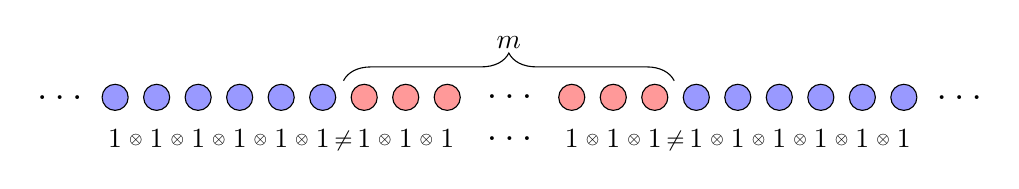
\begin{tikzpicture}[node distance = 15pt, auto]
    \tikzstyle{line} = [draw, -latex',thick]
    \tikzstyle{site1}=[circle, draw, fill=blue!40]
    \tikzstyle{site2}=[circle, draw, fill=red!40]
      % Place nodes

    \node [site1] (site-1) at (-8, 0) {};
    \foreach \x / \name in {1/2,2/3,3/4,4/5,5/6}      
      \node [site1, right of=site-\x] (site-\name) {};

    \node [site2, right of =site-6] (site-7){};
    \foreach \x / \name in {7/8,8/9}      
      \node [site2, right of=site-\x] (site-\name) {};

    \node [site2, right of=site-9, node distance=45pt] (site-10){};
    \foreach \x / \name in {10/11,11/12}      
      \node [site2, right of=site-\x] (site-\name) {};

    \node[site1, right of=site-12] (site-13){};
    \foreach \x / \name in {13/14,14/15,15/16,16/17,17/18}      
      \node [site1, right of=site-\x] (site-\name) {};

    \node [left of=site-1, node distance=20pt] {\Large $ \ldots $};
    \node [right of=site-18, node distance=20pt] {\Large $ \ldots $};
    
      
    \foreach \x in {1,...,18}     
      \node [black, below of=site-\x](op-\x) {\(\mathbb{1}\)};

    \foreach \x / \y in {1/2,2/3,3/4,4/5,5/6,7/8,8/9,10/11,11/12,13/14,14/15,15/16,16/17,17/18}
      \path[draw=none] (op-\x) -- (op-\y) node [black,midway,yshift=-6pt] {\tiny$\otimes$};
    
    \path[draw=none] (op-6) -- (op-7) node [black,midway,yshift=-8pt] {\footnotesize$\neq$};
    \path[draw=none] (op-12) -- (op-13) node [black,midway,yshift=-8pt] {\footnotesize$\neq$};
    % \foreach \x in {-1.5,-1.0,-0.5,0.5,1.0,1.5}
      % \node [site2] (site-\x) at (\x, 0) {};
      
      \draw [decorate,decoration={brace,amplitude=10pt},yshift=6pt] 
      (-5.1,0) -- (-0.9,0) node [black,midway,yshift=8pt] {$m$};
      
      \path [draw=none] (site-9) -- (site-10) node [black,midway,yshift=-4pt] {\Large$\ldots$};
      \path [draw=none] (op-9) -- (op-10) node [black,midway,yshift=-4pt] {\Large$\ldots$};
    \end{tikzpicture}
  \caption{Illustration of an operator supported on \(m\) sites.}
  \label{fig:1D chain}
\end{figure}
In Section~\ref{sec:algorithm}, a precise definition of locality and quasilocality will be stated.


\textcolor{blue}{ Here about commuting and noncommuting operators}

\section{Spectral function \label{sec:spectral function}}

\section{(Q)LIOMs finding algorithm \label{sec:algorithm}}
  \paragraph{}Consider the vector space \(\mathcal{V}_L\) of traceless and translationally invariant observables, acting on a Hilbert space of dimension \(2^L\). We can define an inner
  product on this space:
  \begin{equation}
      \left(A|B\right) = \frac{1}{2^L}\tr(A^{\dagger}B) = \frac{1}{2^L} \sum_{mn} A_{nm}B_{nm}^{\ast}
  \end{equation}
  i.e. the Hilbert-Schmidt product, where \(A_{nm} = \matrixel{n}{A}{m}\) and \(H\ket{n} = E_n \ket{n}\). This definition is correct, as we work only with finite dimensional Hilbert spaces. We require the operators to be traceless, becauese they
  have zero overlap with the identity, \(\left(A|\Id\right)=\frac{1}{2^L}\tr(A) = 0\).
  
  
  
  Now we introduce an orthonormal basis of \({\mathcal{A}_L^m}\):
  \begin{equation}
      O_{\underline{s} } = \sum_{j = 1}^L \sigma_{j}^{s_1}\sigma_{j+1}^{s_2}\cdots \sigma_{j+m-1}^{s_m}
  \end{equation}
  where \(\sigma^z_j \equiv \sqrt{2}S^{z}_j\), \(\sigma^{\pm}_j \equiv S^{\pm}_j\), \(\sigma^0_j\equiv \Id\), \(\underline{s} = (s_1,s_2,\ldots s_m)\)
  and \(s_j \in \{+,-,z,0\}\) while \(s_{1,m} \in \{+,-,z\}\). For a fixed m, there are exactly \(N_m = 3\cdot 4^{m-2}\cdot 3\) such operators and they
  satisfy an orthonormality condition i.e \(\left(O_{\underline{s}}|O_{\underline{s'}}\right) = \delta_{\underline{s},\underline{s'}}\). 
  
  We define the infinite time averaging of an operator \(A\in \mathcal{A}_L^m\), employing the Heisenberg picture:
  \begin{align}
  \overline{A} = &\lim_{\tau \rightarrow \infty} \frac{1}{\tau} \int dt\, A_{H}(t) =  \nonumber
  \lim_{\tau \rightarrow \infty} \frac{1}{\tau} \int dt\, e^{i H t}A e^{-i H t} = \\ \nonumber
  &\sum_{n,m} \lim_{\tau \rightarrow \infty} \frac{1}{\tau} \int dt\, e^{i E_m t}\ket{m}  
  \matrixel{m}{A}{n}\bra{n}  e^{-i E_n t} = \\ 
  & \sum_{n,m} \matrixel{m}{A}{n}\ketbra{m}{n} \lim_{\tau \rightarrow \infty} \frac{1}{\tau}
  \int dt \, e^{i(E_m-E_n)t} =  \sum_{n,m}^{E_n = E_m} \matrixel{m}{A}{n}\ketbra{m}{n}
  \label{eq:time_avg}
  \end{align}
  It is evident from equation~\eqref{eq:time_avg} that large degeneracy of energy spectrum will be important to the
  structure of time-averaged operators. Moreover, time averaging in such form is an orthogonal projection in the
  Hilbert space of operators. From that follows a crucial property i.e \(\left(\overline{A}|\overline{B}\right) = 
  \left(\overline{A}|B\right)\).
  
  \textcolor{blue}{Here continues a detailed derivation of the algorithm. And something about fermions.}
  Operators with corresponding to largest eigenvalues of \(K\) matrix 
  


  \section{Algorithm}
